\documentclass[12pt,letterpaper]{article}
\usepackage[utf8]{inputenc}
\usepackage[spanish]{babel}
\usepackage{graphicx}
\usepackage[left=2cm,right=2cm,top=2cm,bottom=2cm]{geometry}
\usepackage{graphicx} % figuras
% \usepackage{subfigure} % subfiguras
\usepackage{float} % para usar [H]
\usepackage{amsmath}
%\usepackage{txfonts}
\usepackage{stackrel} 
\usepackage{multirow}
\usepackage{enumerate} % enumerados
\renewcommand{\labelitemi}{$-$}
\renewcommand{\labelitemii}{$\cdot$}
% \author{}
% \title{Caratula}
\begin{document}

% Fancy Header and Footer
% \usepackage{fancyhdr}
% \pagestyle{fancy}
% \cfoot{}
% \rfoot{\thepage}
%

% \usepackage[hidelinks]{hyperref} % CREA HYPERVINCULOS EN INDICE

% \author{}
\title{Caratula}

\begin{titlepage}
\begin{center}
\large{UNIVERSIDAD PRIVADA-DE-TACNA}\\
\vspace*{-0.025in}
\begin{figure}[htb]
\begin{center}

\includegraphics[width=8cm]{./Imagenes/logo}
\end{center}
\end{figure}
\vspace*{0.15in}
INGENIERIA DE SISTEMAS  \\

\vspace*{0.5in}
\begin{large}
TITULO:\\
\end{large}

\vspace*{0.1in}
\begin{Large}
\textbf{Modelando Datos en Power BI} \\
\end{Large}

\vspace*{0.3in}
\begin{Large}
\textbf{CURSO:} \\
\end{Large}

\vspace*{0.1in}
\begin{large}
Inteligencia de Negocios\\
\end{large}

\vspace*{0.3in}
\begin{Large}
\textbf{DOCENTE(ING):} \\
\end{Large}

\vspace*{0.1in}
\begin{large}
 Patrick Cuadros Quiroga\\
\end{large}

\vspace*{0.2in}
\vspace*{0.1in}
\begin{large}
Integrante: \\
\begin{flushleft}
Rivas Rios, Marko Antonio          	\hfill	(2016054461) \\

\end{flushleft}
\end{large}
\end{center}

\end{titlepage}


\tableofcontents % INDICE
\thispagestyle{empty} % INDICE SIN NUMERO
\newpage
\setcounter{page}{1} % REINICIAR CONTADOR DE PAGINAS DESPUES DEL INDICE

\section{Proceso} 

\textbf{Ejercicio 1: Crear relaciones}

\begin{itemize}
	\item En el cuadro de dialogo Explorador, seleccionar las hojas DimCurrency, DimCustomer, DimDate, DimProduct, DimPromotion, DimSalesTerritory, y FactInternetSales.
	\begin{center}
	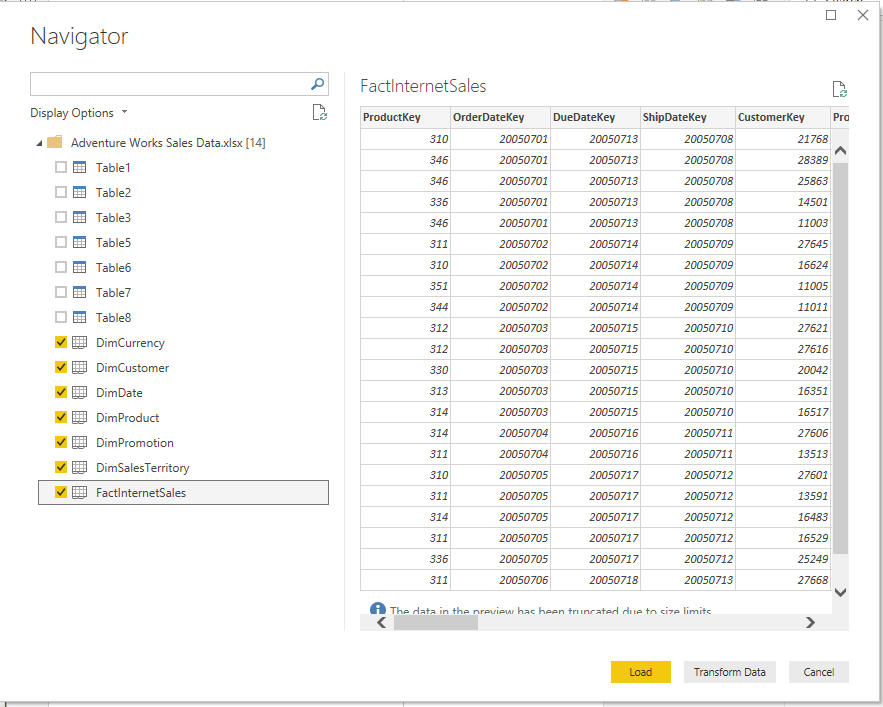
\includegraphics[width=10cm]{./Imagenes/Captura1} 
	\end{center}
\end{itemize} 

\begin{itemize}
	\item Vista Fields de las hojas seleccionadas.
	\begin{center}
	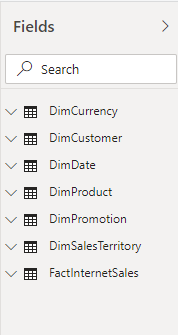
\includegraphics[width=5cm]{./Imagenes/Captura2} 
	\end{center}
\end{itemize} 

\begin{itemize}
	\item  Panel de modelamiento.
	\begin{center}
	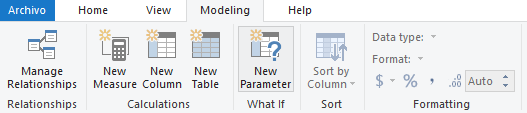
\includegraphics[width=10cm]{./Imagenes/Captura3} 
	\end{center}
\end{itemize} 

\begin{itemize}
	\item Cuadro de Administrar relaciones (Manage Relationships).
	\begin{center}
	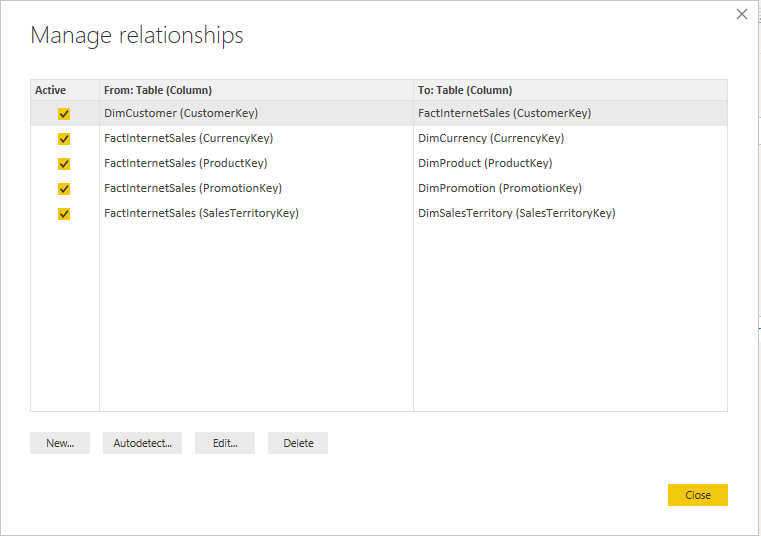
\includegraphics[width=10cm]{./Imagenes/Captura4} 
	\end{center}
\end{itemize} 

\begin{itemize}
	\item Creado una nueva relacion en el cuadro de Administrar relaciones.
	\begin{center}
	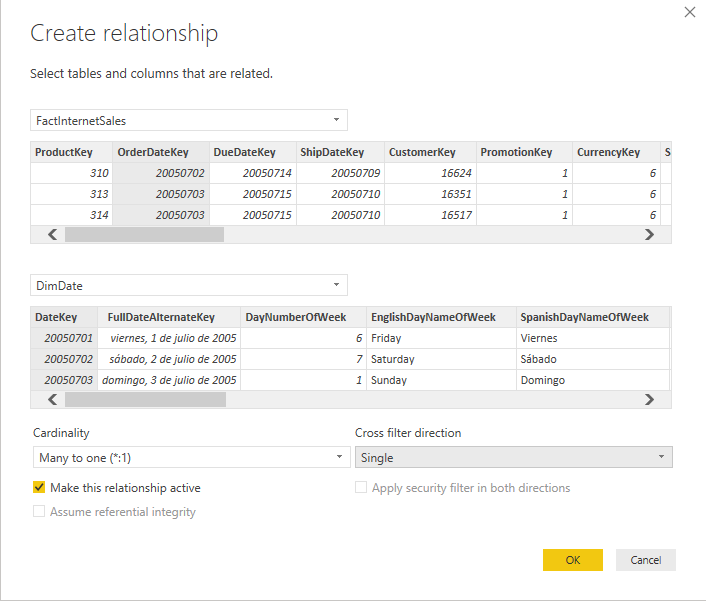
\includegraphics[width=10cm]{./Imagenes/Captura5} 
	\end{center}
\end{itemize} 

\begin{itemize}
	\item Vista de Modelo de todas las relaciones.
	\begin{center}
	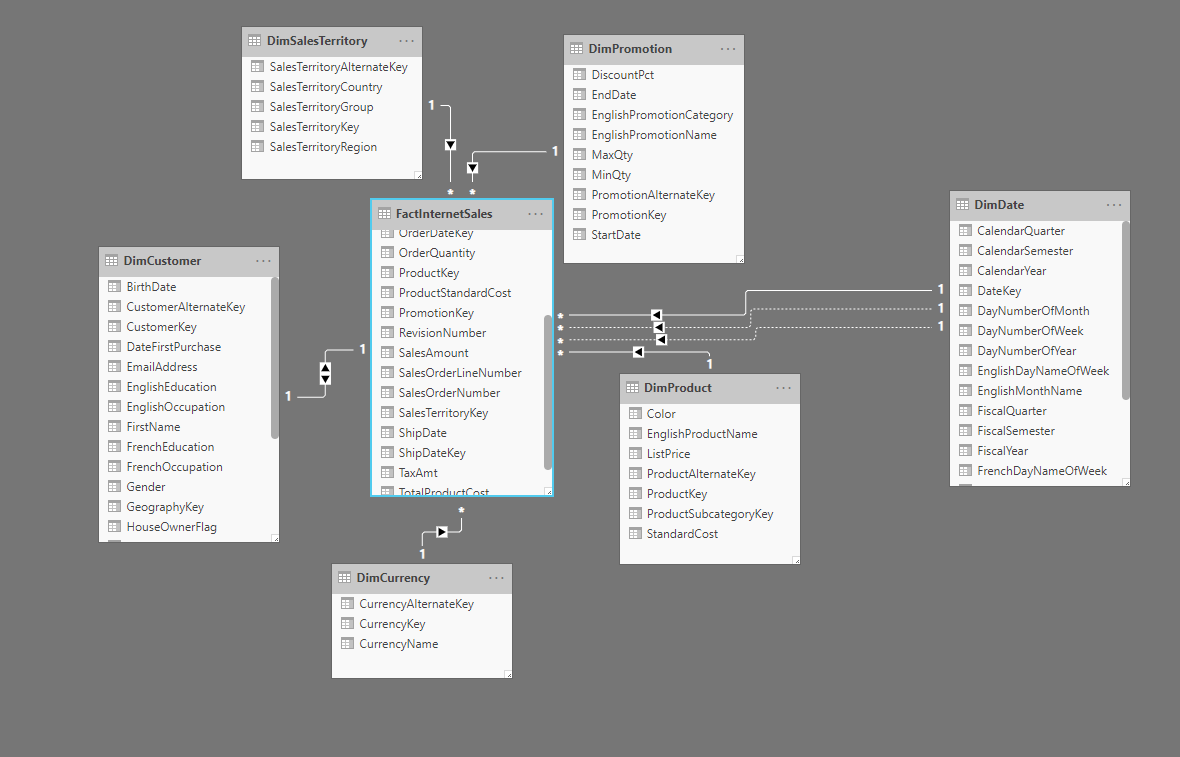
\includegraphics[width=13cm]{./Imagenes/Captura6} 
	\end{center}
\end{itemize} 

\begin{itemize}
	\item Eliminar la línea de la relación entre DimProductCategory, y DimProductSubcategory.
	\begin{center}
	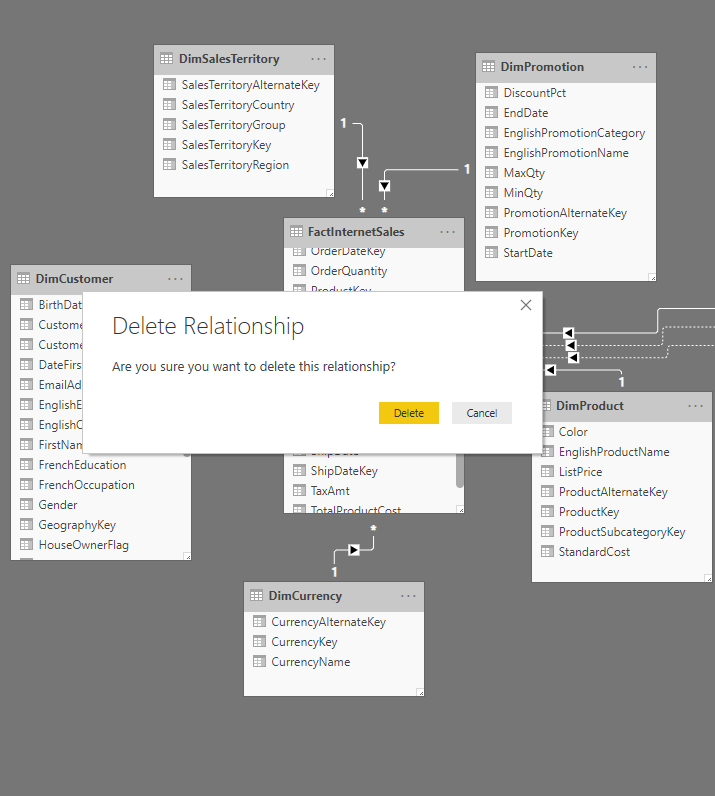
\includegraphics[width=13cm]{./Imagenes/Captura7} 
	\end{center}
\end{itemize} 
\begin{itemize}
	\item Creando una nueva relacion entre FactInternetSales y CustomerKey.
	\begin{center}
	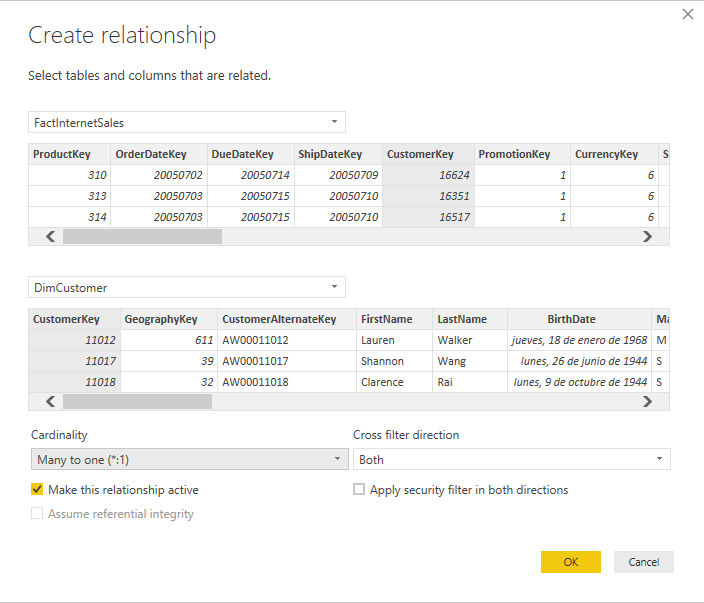
\includegraphics[width=13cm]{./Imagenes/Captura8} 
	\end{center}
\end{itemize} 


\textbf{Ejercicio 2: Relaciones manuales}


\begin{itemize}
	\item cuadro de dialogo Explorador, seleccionar las hojas DimProductCategory, y DimProductSubcategory.
	\begin{center}
	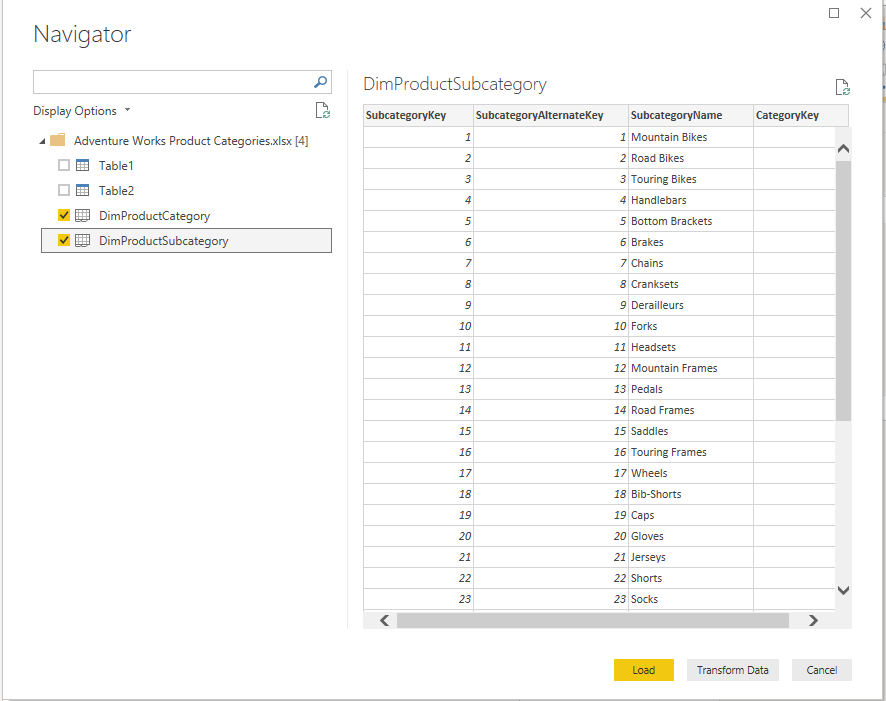
\includegraphics[width=13cm]{./Imagenes/Captura2-1} 
	\end{center}
\end{itemize} 

\begin{itemize}
	\item Vista de Modelo de la relacion.
	\begin{center}
	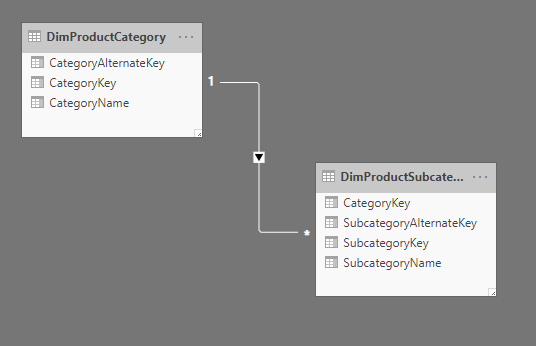
\includegraphics[width=13cm]{./Imagenes/Captura2-2} 
	\end{center}
\end{itemize} 

\begin{itemize}
	\item Eliminando la línea de la relación entre DimProductCategory, y DimProductSubcategory.
	\begin{center}
	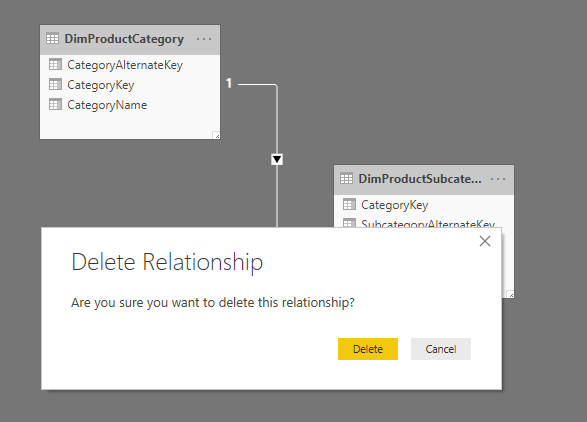
\includegraphics[width=13cm]{./Imagenes/Captura2-3} 
	\end{center}
\end{itemize} 

\begin{itemize}
	\item Creando la relacion entre la columna ProductSubcategoryKey a la columna SubcategoryKey en la tabla DimProductSubcategory, para crear una relación de Muchos a Uno (Many to One (*:1)), y una dirección de filtro cruzado (Cross filter direction) en ambos.
	\begin{center}
	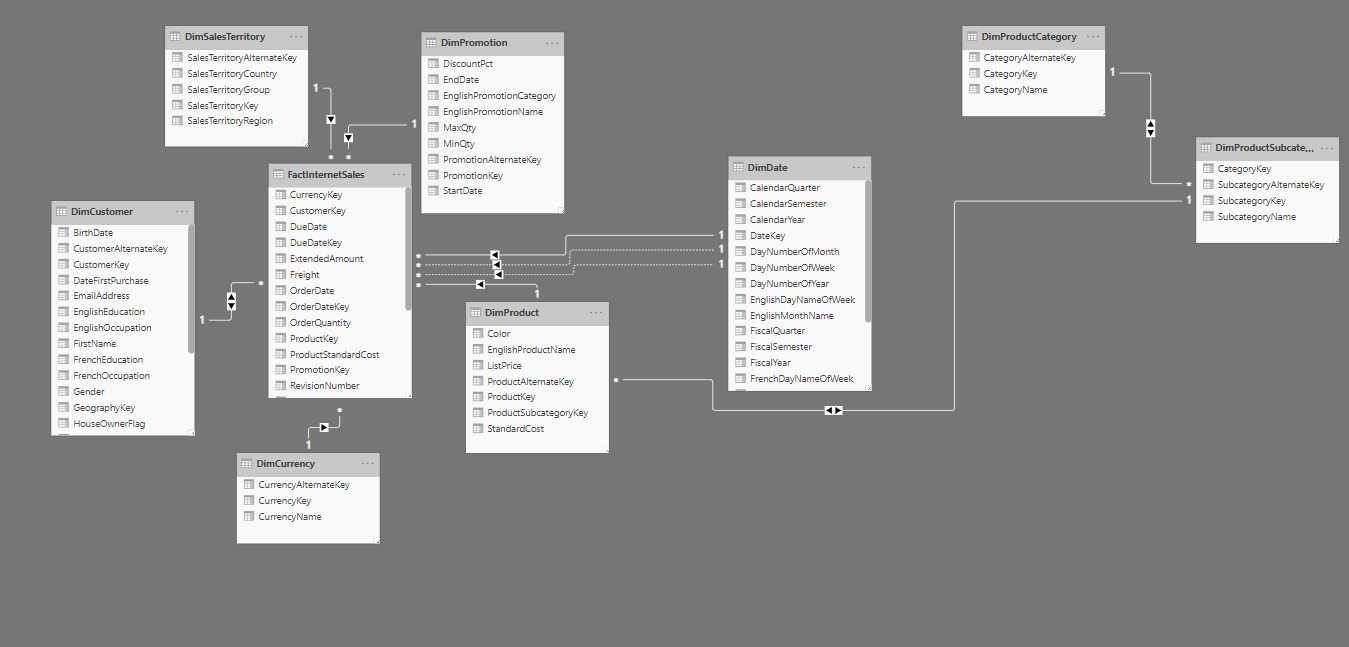
\includegraphics[width=13cm]{./Imagenes/Captura2-4} 
	\end{center}
\end{itemize} 


\textbf{Ejercicio 3: Cálculos}


\begin{itemize}
	\item Vista Data.
	\begin{center}
	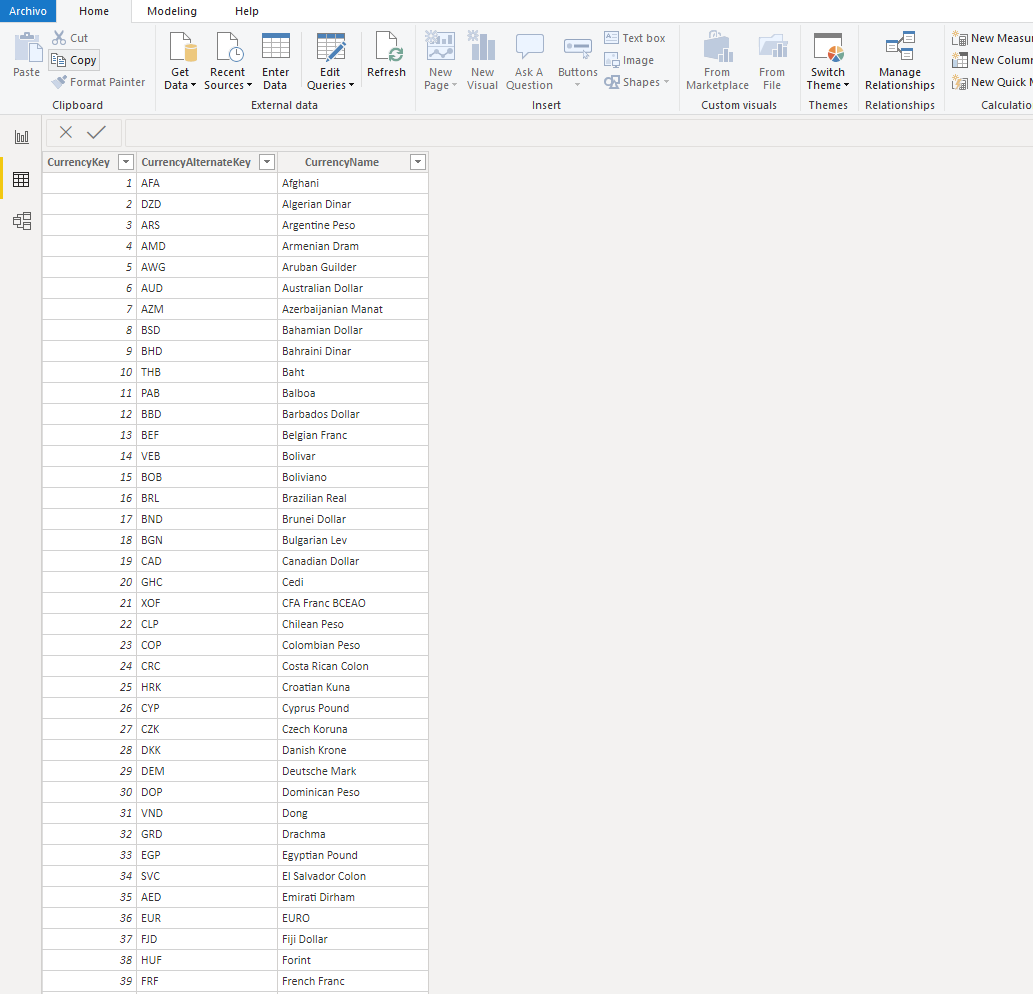
\includegraphics[width=13cm]{./Imagenes/Captura3-1} 
	\end{center}
\end{itemize} 

\begin{itemize}
	\item Vista Data de DimCustomer.
	\begin{center}
	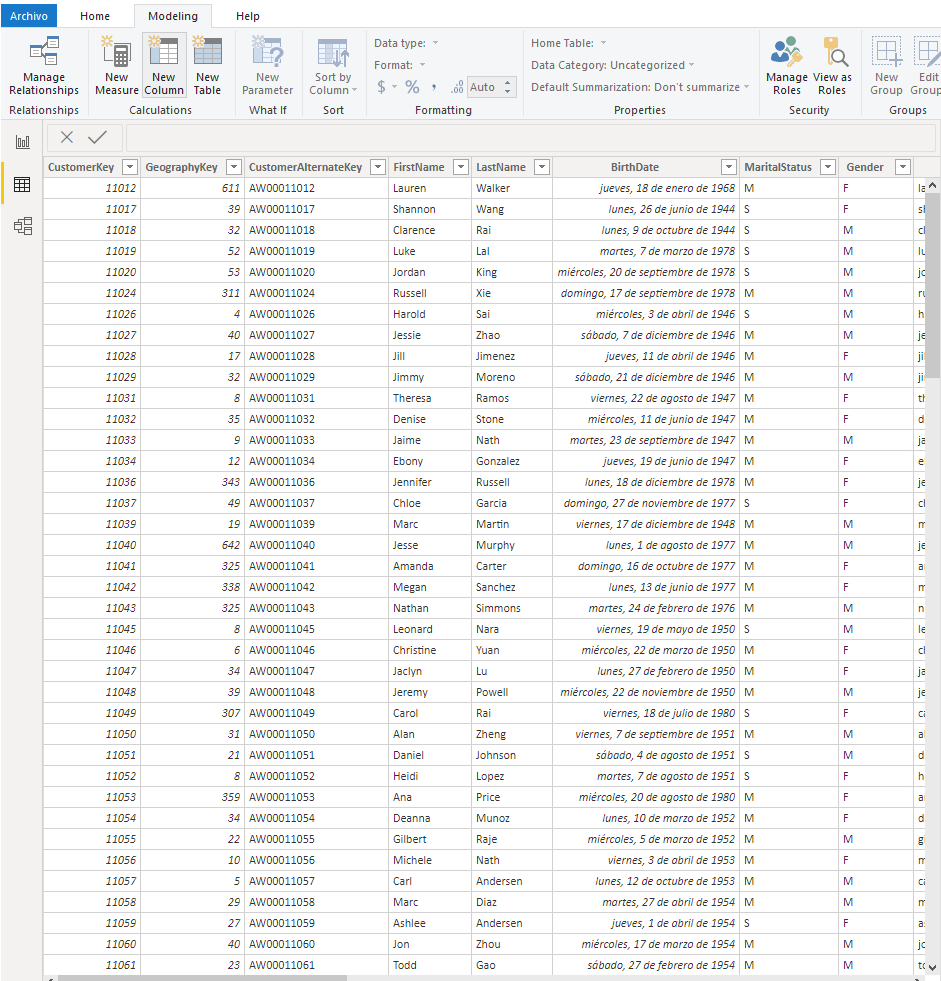
\includegraphics[width=13cm]{./Imagenes/Captura3-2} 
	\end{center}
\end{itemize} 

\begin{itemize}
	\item Nuevas columnas creadas, IncomeStatus, DaysSinceFirstPurchase, FullName, MaleFemale, Relationship.
	\begin{center}
	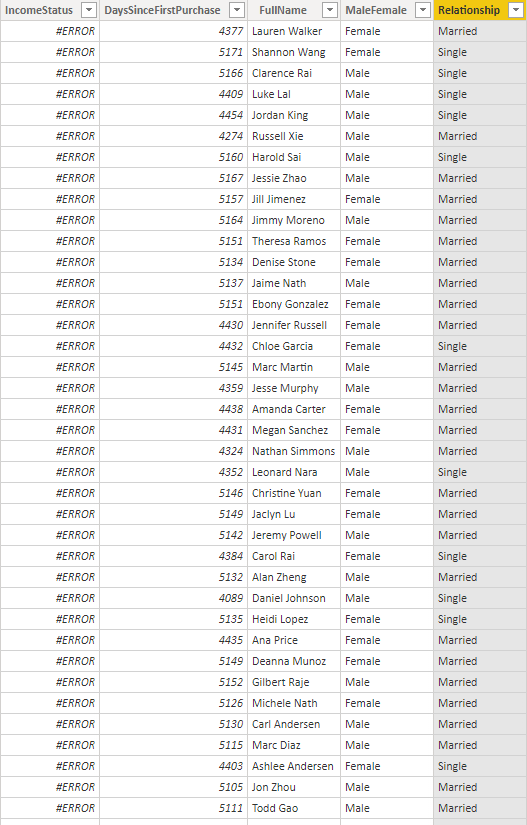
\includegraphics[width=10cm]{./Imagenes/Captura3-3} 
	\end{center}
\end{itemize} 

\begin{itemize}
	\item creando la columna MainCategory.
	\begin{center}
	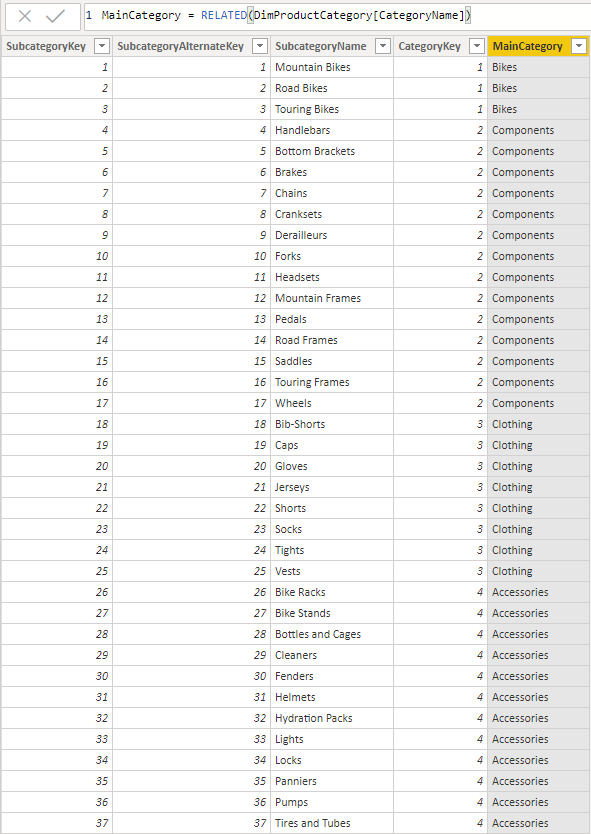
\includegraphics[width=10cm]{./Imagenes/Captura3-4} 
	\end{center}
\end{itemize}

\begin{itemize}
	\item creando la columna PromotionLengthDays.
	\begin{center}
	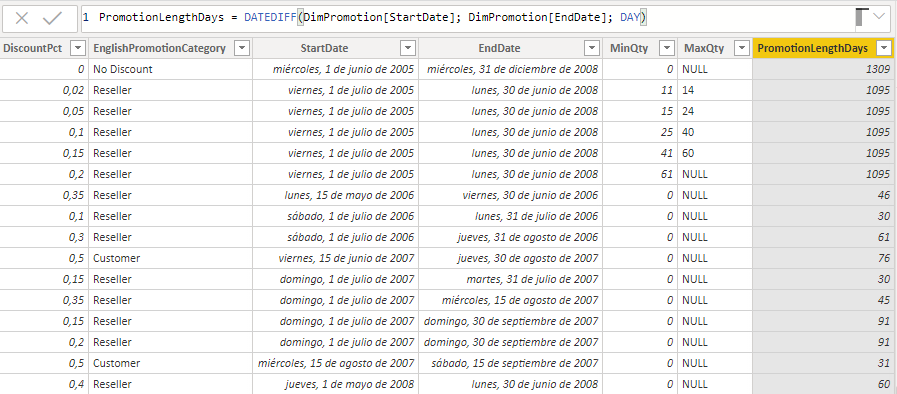
\includegraphics[width=10cm]{./Imagenes/Captura3-5} 
	\end{center}
\end{itemize}

\begin{itemize}
	\item creando la columna Profit.
	\begin{center}
	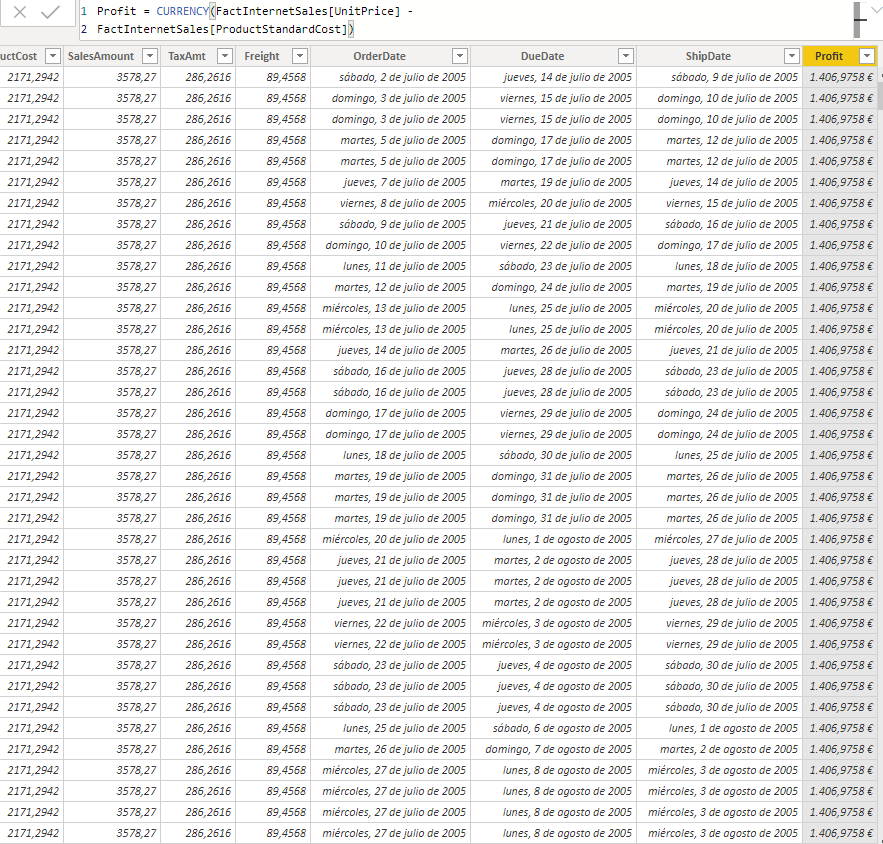
\includegraphics[width=10cm]{./Imagenes/Captura3-6} 
	\end{center}
\end{itemize}












\end{document}
